\section{Virtual Reality}
With the launch and success of modern technologies like Oculus Rift, HTC Vive or Playstation VR (Figure \ref{fig:CONTROLLERS}), today’s virtual reality (VR) is mostly associated with a head-mounted device that provides this experience for the wearer. Virtual reality headsets combine a stereoscopic head-mounted display (HMD), stereophonic sound, and sensors like gyroscopes or accelerometers for head motion tracking. The main goal of these devices is to fool user’s senses, make him feel present and immersed in virtual reality. A person using such equipment is able to move and look around artificial world. Usually users can also interact with its features in some way, using specially designed controllers. Today VR headsets are mostly used for gaming, simulations, education, and other entertainment purposes.

\begin{figure}[th]
\centering
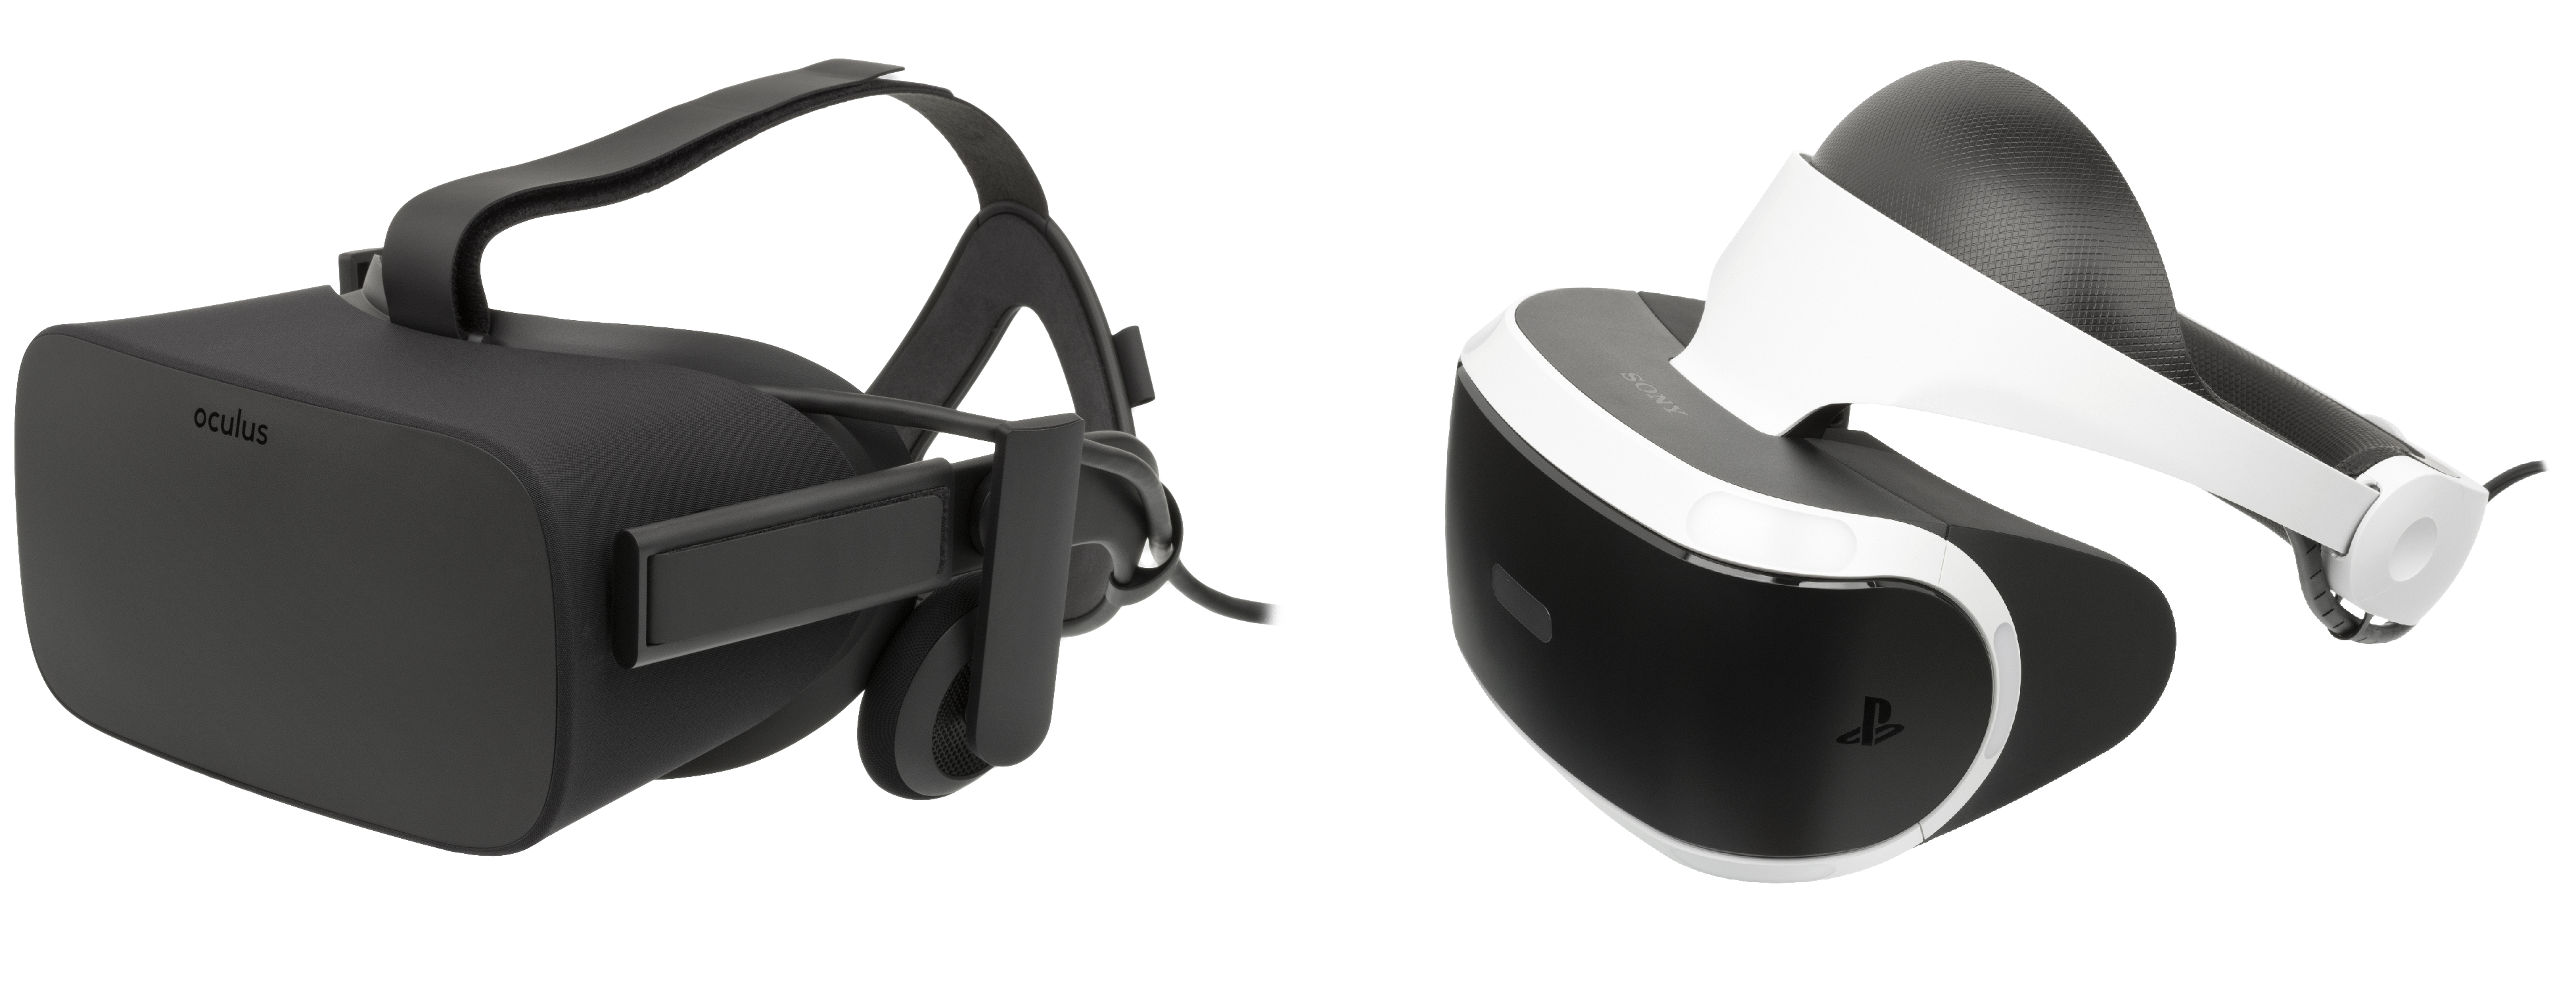
\includegraphics[width=1\textwidth]{img/headsets.png}
\caption{Modern popular VR headsets: Oculus Rift and Playstation VR (source: \cite{OCULUS_HEADSET}\cite{PSVR_HEADSET})}
\label{fig:CONTROLLERS}
\end{figure}

The concept of virtual reality is evolving and changing quickly. The technologies we use now will probably become obsolete in next 5 years. To describe what virtual Reality really means, we must be broad enough to enclose what it meant in the past, what it is today, and what it can become in the future. S. M. LaValle in his book \cite{VR_BOOK} tries this approach to define VR in general way. The four key concepts which appear in his VR definition are:

\begin{itemize}
\item \textit{Targeted behavior}: The experience from the real world we try to replicate. It could be anything from walking, dancing, swimming, shooting arrows, etc.
\item \textit{Organism}: Any life form can be the user of VR. In the past it was tested even on animals like cockroaches, fishes, monkeys and rodents.
\item \textit{Artificial sensory stimulation}: With the use of available equipment and technology, organism’s senses are tricked to make him feel present in artificial reality.
\item \textit{Awareness}: While being immersed in VR, the user should be oblivious to any interference. Feeling presence in this altered or another world is accepted as natural.
\end{itemize}

Virtual reality has a long history and can be traced back even to 1962, when Morton Heilig built a machine called Sensorama \cite{SENSORAMA}. It could provide body tilting, supply stereo sound, display stereoscopic 3-D images, and was able to trigger tracks of aromas and wind during the film. Later in 1968, Ivan Sutherland invented what is regarded as the first head-mounted display device: The Sword of Damocles \cite{DAMOCLES}. The system provided basic user interface and realism, the graphics of created VR were simple wire-frame model rooms. The device was so heavy that it had to be attached to the ceiling with a mechanical arm (Figure \ref{fig:FIRST_VR}). In the next years VR devices were mainly used for flight simulation, military training, medical purposes and automobile design. Advancements in technology and the launch of an affordable high-quality VR headsets, made virtual reality more accessible for video game players. Today we are witnessing an exciting rebirth of interest in VR, not only in entertainment industry but also in academic research.

\begin{figure}[th]
\centering
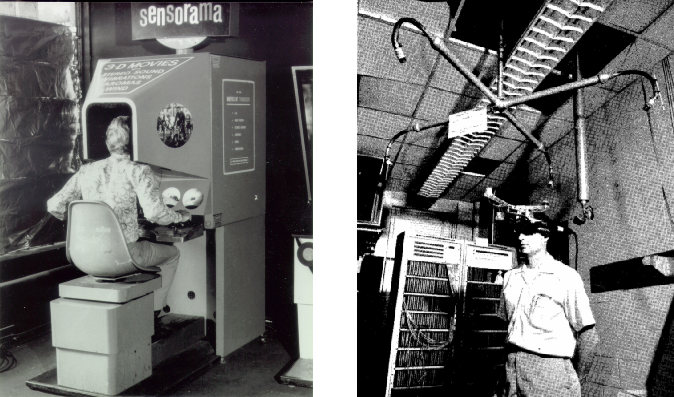
\includegraphics[width=1\textwidth]{img/first_vr.png}
\caption{The Sensorama and The Sword of Damocles, first attempts at creating virtual reality (source: \cite{SENSORAMA_IMAGE}\cite{DAMOCLES})}
\label{fig:FIRST_VR}
\end{figure}

\section{VR input methods}

As more companies enter the VR headset market, we can see the rapid technological advancement in input devices. Authors of the article \textit{State of the Art of Virtual Reality Technology} \cite{VR_TECHNOLOGY} identified three different categories for devices handling input in VR: controllers, navigation devices and tracking technologies. Most of the controllers for VR headsets are hand worn and provide 6DoF (Six Degrees of Freedom) tracking information. They are usually equipped with buttons for discrete input, and top-mounted touchpads or joysticks for analog input (Figure \ref{fig:CONTROLLERS_IMAGE}).

\begin{figure}[th]
\centering
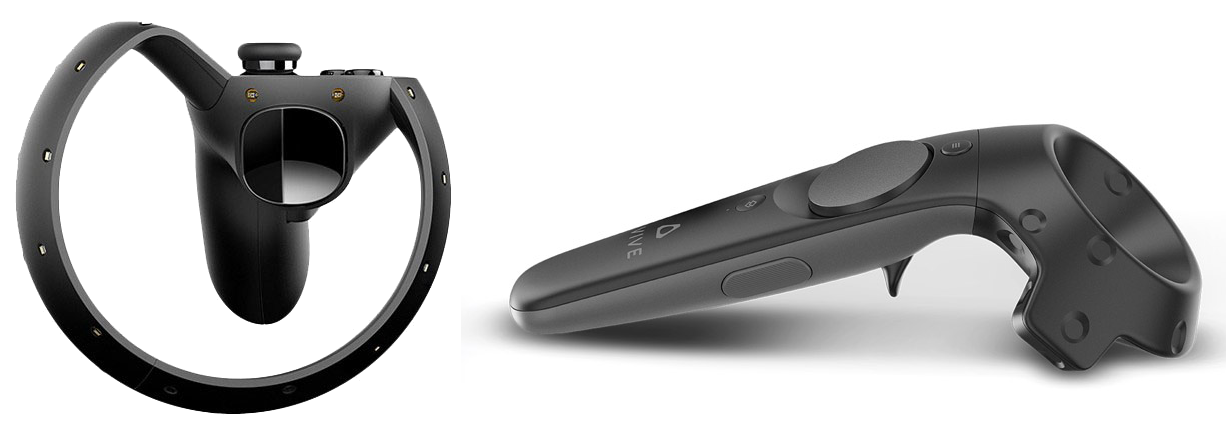
\includegraphics[width=1\textwidth]{img/modern_controllers.png}
\caption{Modern VR controllers: The Oculus Touch and HTC Vive Controller (source:  \cite{VR_TECHNOLOGY}\cite{VIVE_IMAGE})}
\label{fig:CONTROLLERS_IMAGE}
\end{figure}

The illusion of traversing an endless space can be achieved with the help of navigation devices which are an input source for moving in the virtual environment. Most devices in this category act similar to traditional treadmills allowing movement in one direction. Some of them allow motion on a two-dimensional plane or function like the slidemills. For example, Virtuix Omni (Figure \ref{fig:VIRTUX_IMAGE}) is a concave platform with a low-friction surface which allows locomotive motion in any direction. There are also attempts at creating devices less expensive and more affordable to general public. Google is currently working on motorized shoes that allow an endless movement in a limited space \cite{VR_SHOES}. Other researchers try to use devices which were not specially designed for virtual reality. For instance, A. Aguirre in his master thesis \cite{JOYSTICK} describes the process of navigation in VR through leaning on Wii Balance Board.

\begin{figure}[th]
\centering
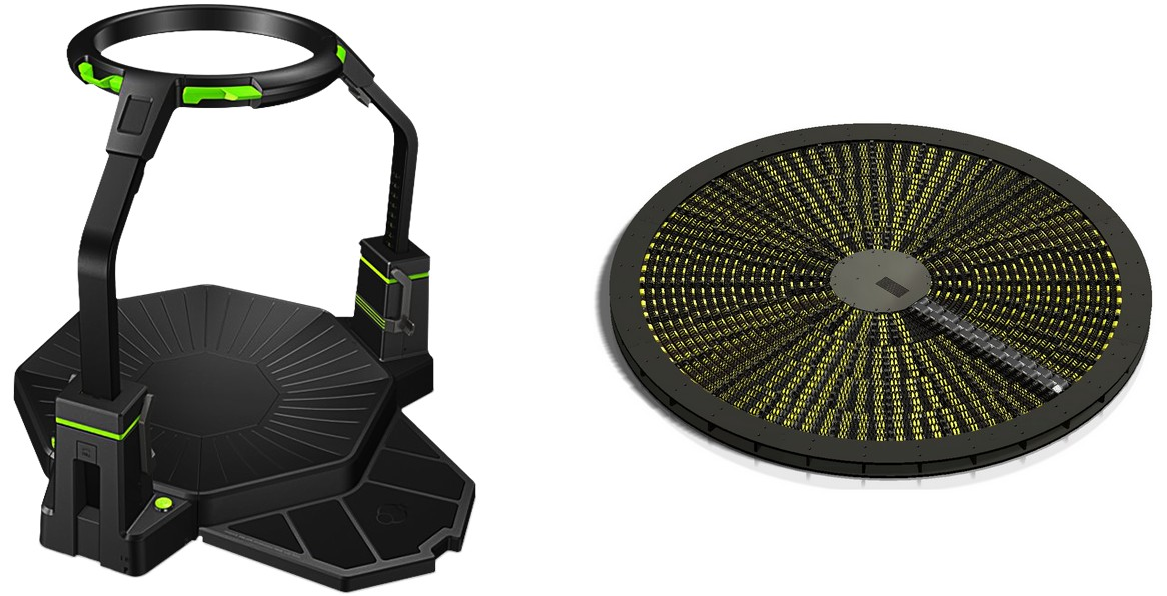
\includegraphics[width=0.9\textwidth]{img/vr_threadmills.png}
\caption{Examples of omnidirectional treadmills: Virtuix Omni and WalkMouse (source:  \cite{VR_TECHNOLOGY})}
\label{fig:VIRTUX_IMAGE}
\end{figure}

There are currently two approaches for motion tracking technologies. First is full body tracking which focuses on posture and upper body of the users. Second is gesture tracking which is usually achieved optically or with devices worn on hands. Full body tracking is commonly implemented using magnetic tracking or Inertial Measurement Units (IMUs), providing six degrees of freedom by placing orthogonally to each other accelerometers, gyroscopes and magnetometers. Valve came up with different approach, their Lighthouse positional tracking system involves two base stations \cite{VIVE_STATION} that scan the area around room with lasers. There are also various sensor technologies designed to be worn like a glove which are used to capture gestures such as bending of fingers. One of these data gloves called Gloveone \cite{GLOVEONE}, enables users to feel and touch any virtual object that they can see in VR headsets. There are 10 actuators distributed along the fingertips and palm of the glove, which vibrate independently at different intensities and frequencies, reproducing touch sensations.

\section{Locomotion in VR}




